\documentclass[UTF8,a4paper,10pt]{ctexart}
\usepackage[left=2.50cm, right=2.50cm, top=2.50cm, bottom=2.50cm]{geometry}
%页边距
\CTEXsetup[format={\Large\bfseries}]{section} %设置章标题居左

%%%%%%%%%%%%%%%%%%%%%%%
% -- text font --
% compile using Xelatex
%%%%%%%%%%%%%%%%%%%%%%%
% -- 中文字体 --
%\setmainfont{Microsoft YaHei}  % 微软雅黑
%\setmainfont{YouYuan}  % 幼圆    
%\setmainfont{NSimSun}  % 新宋体
%\setmainfont{KaiTi}    % 楷体
%\setmainfont{SimSun}   % 宋体
%\setmainfont{SimHei}   % 黑体
% -- 英文字体 --
%\usepackage{times}
%\usepackage{mathpazo}
%\usepackage{fourier}
%\usepackage{charter}

%\usepackage{helvet}

\usepackage{amsmath, amsfonts, amssymb} % math equations, symbols
\usepackage[english]{babel}
\usepackage{color}	% color content
\usepackage{graphicx}	% import figures
\usepackage{url}	% hyperlinks
\usepackage{bm} 	% bold type for equations
\usepackage{multirow}
\usepackage{booktabs}
\usepackage{epstopdf}
\usepackage{epsfig}
\usepackage{algorithm}
\usepackage{algorithmic}
\usepackage{listings}
\usepackage{xcolor}
\usepackage{booktabs}
\usepackage{zhnumber}
\usepackage{longtable}
\usepackage{subfigure}
\usepackage{float}
\usepackage{caption}
\usepackage{subfigure}
\renewcommand\thesection{\zhnum{section}}
\renewcommand \thesubsection {\arabic{section}}
\renewcommand{\algorithmicrequire}{ \textbf{Input:}}
% use Input in the format of Algorithm  
\renewcommand{\algorithmicensure}{ \textbf{Initialize:}}
% use Initialize in the format of Algorithm  
\renewcommand{\algorithmicreturn}{ \textbf{Output:}}
% use Output in the format of Algorithm  
%%%%%%%%%%%%%%%%%%
\usepackage{listings}
\usepackage{color}
\definecolor{dkgreen}{rgb}{0,0.6,0}
\definecolor{gray}{rgb}{0.5,0.5,0.5}
\definecolor{mauve}{rgb}{0.58,0,0.82}
\lstset{frame=tb,
  language=Python,
  aboveskip=3mm,
  belowskip=3mm,
  showstringspaces=false,
  columns=flexible,
  basicstyle={\small\ttfamily},
  numbers=left,%设置行号位置none不显示行号
  %numberstyle=\tiny\courier, %设置行号大小
  numberstyle=\tiny\color{gray},
  keywordstyle=\color{blue},
  commentstyle=\color{dkgreen},
  stringstyle=\color{mauve},
  breaklines=true,
  breakatwhitespace=true,
  escapeinside=``,%逃逸字符(1左面的键),用于显示中文例如在代码中`中文...`
  tabsize=4,
  extendedchars=false %解决代码跨页时,章节标题,页眉等汉字不显示的问题
}

%%%%%%%%%%%%%%%%%%%%%%%%%%%%
\usepackage{fancyhdr} %设置页眉、页脚
\pagestyle{fancy}
\lhead{}
\chead{}
%\rhead{\includegraphics[width=1.2cm]{fig/ZJU_BLUE.eps}}
\lfoot{}
\cfoot{}
\rfoot{}
\fancyfoot[RE,RO]{~\thepage~}

\fancyhead[RE,RO]{计算物理导论 \quad 2022春季学期 \quad 作业6  \quad 何翼成}

%%%%%%%%%%%%%%%%%%%%%%%
%  设置水印
%%%%%%%%%%%%%%%%%%%%%%%
%\usepackage{draftwatermark}         % 所有页加水印
%\usepackage[firstpage]{draftwatermark} % 只有第一页加水印
% \SetWatermarkText{Water-Mark}           % 设置水印内容
% \SetWatermarkText{\includegraphics{fig/ZJDX-WaterMark.eps}}         % 设置水印logo
% \SetWatermarkLightness{0.9}             % 设置水印透明度 0-1
% \SetWatermarkScale{1}                   % 设置水印大小 0-1    

\usepackage{hyperref} %bookmarks
\hypersetup{colorlinks, bookmarks, unicode} %unicode

\title{\textbf{龙格库塔法求解微分方程}}
\author{ 何翼成 \thanks{学号:520072910043; \newline
    邮箱地址:heyicheng@sjtu. edu. cn} }
\date{\today}

\begin{document}
\maketitle

%\begin{abstract}
%这是一篇中文小论文。这个部分用来写摘要。摘要的章标题默认是英文,还没找到改成中文的方法:(
%\end{abstract}
\section*{Project 1}
\section{题目分析}
%%%以下为插入图片模板
%\quad \newline
	\begin{figure}[!htbp]
		\centering
		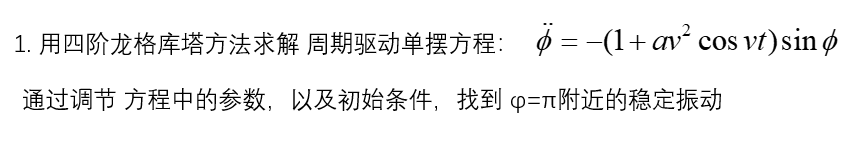
\includegraphics[width=1\textwidth,height=0.2\textwidth]{pictures/project1.png}
		\caption{题目总览} \label{project1}
	\end{figure}
  由上可知,即可构造$y_{1}=\phi ,y_{2}=y_{1}^{'}$,从而使用龙科库塔法
  进行数值求解


\section{代码展示}

\subsubsection{前置函数编写}
以下为第一问所用到的微分方程,通过构造写为方程组,不难知道该问题为2阶。\newline
~\\
\lstset{language=matlab}
\begin{lstlisting}
  %编写第一问的方程组,由于本问题的阶数为2所以以下按照2阶编写
  %为了方便表示,将原始方程简写为以下形式:
  %y''=-(1+a*v^2*cos(v*x))*sin(y)
  %令y=y(1),y'=y(2),y''=y(2)'
  %初始条件为y(0)=pi,y'(0)=?(待定系数)
  function dy=Fun(x,y)
  %x为自变量
  %y为向量,包含y,y',y''...等
  %a,v为待定的方程参数
  a=1;v=0.01;%暂定方程参数a,v
  dy=zeros(size(y));
  dy(1)=y(2);                         %dy(1)即为y的一阶导
  dy(2)=-(1+a*v^2*cos(v*x)).*sin(y(1));%dy(2)即为y的二阶导
  end
\end{lstlisting}
以下则是编写龙格库塔法的主体函数,即使用加权的斜率平均数进行步进法。\newline

~\\
\lstset{language=matlab}
\begin{lstlisting}
  function y=RK(x,h,y)
    len=length(x);%x为行向量
     %龙格库塔法主体函数
    for i=2:len
        K1=Fun(x(i-1),y(i-1,:));                %K1
        K2=Fun(x(i-1)+1/2*h,y(i-1,:)+1/2*h.*K1);%K2
        K3=Fun(x(i-1)+1/2*h,y(i-1,:)+1/2*h.*K2);%K3
        K4=Fun(x(i-1)+h,y(i-1,:)+h.*K3);        %K4
        y(i,:)=y(i-1,:)+h/6.*(K1+2*K2+2*K3+K4);     %更新y的第i行,其中y(i,1)是原函数的y,y(i,2)是原函数的一阶导...
    end
end
\end{lstlisting}
以下为绘图函数,观察$\phi $在一段时间内的震荡情况来判断是否达到了所要求的
“在$\pi$附近震荡”的情况。\newline
~\\
\lstset{language=matlab}
\begin{lstlisting}
  function y=PlotAll()
  x=0:0.001:100;%x:行向量,代表了历经的时间t
  l=length(x);
  h=x(2)-x(1);%h:步长,注意和x的间隔相同
  y=zeros(length(x),2);%y:矩阵,列数为微分方程阶数,行数为x的长度。
  y(1,:)=[pi,5];%代入初始条件,由于是在\Phi=pi附近,所以不妨设初始位置就在pi。
  Y=RK(x,h,y);
  hold on
  grid on
  phi=Y(:,1);
  %区间平移,将其整理在[0,2*pi]区间内
  for ii=1:length(phi)
      while phi(ii)>2*pi
          phi(ii)=phi(ii)-2*pi;
      end
      while phi(ii)<0
          phi(ii)=phi(ii)+2*pi;
      end
  end
  plot(x,phi)
  xlabel('t')
  ylabel('\Phi')
  %添加一条基准线
  plot(x,zeros(1,l)+pi,'k')
  end
\end{lstlisting}
\subsubsection{主体函数编写}
~\\
\lstset{language=matlab}
\begin{lstlisting}
  clear;clc;
  PlotAll()
\end{lstlisting}
由此可以观察得到的图像进行简要分析,从而得到所需要的初始条件和方程参数。
\section{结果分析与结论}
由于尝试思路不明确,所以在得出结论的时候较为困难。在这里进行了
简单的调参,得到了一个看似周期性的结果,所以录入如下。
	\begin{figure}[!htbp]
		\centering
		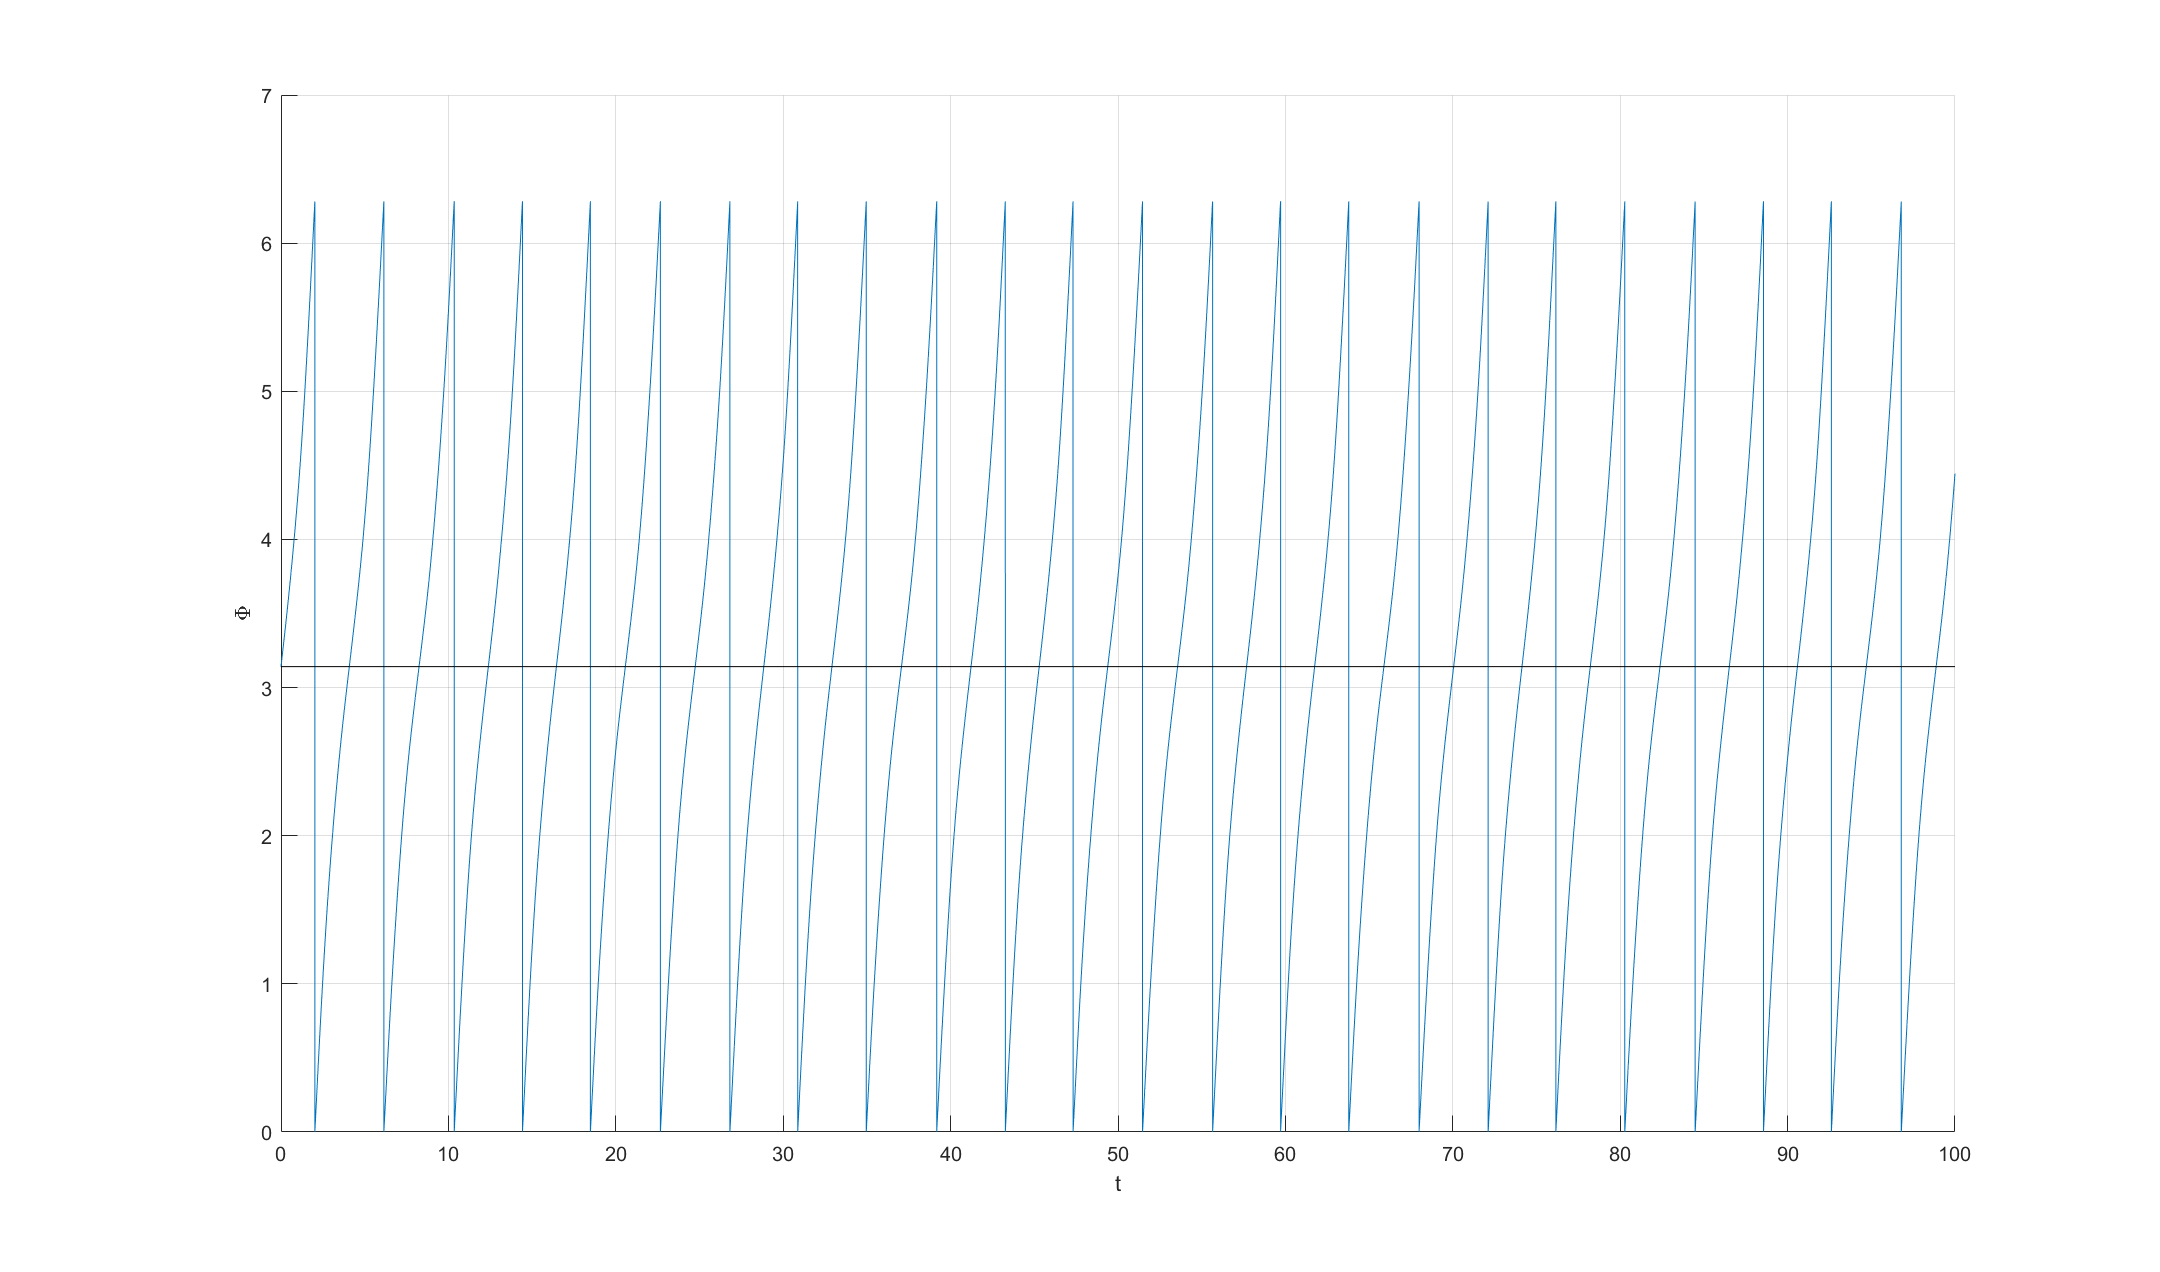
\includegraphics[width=1\textwidth,height=0.75\textwidth]{pictures/p1.png}
		\caption{调参后(a=0.01,v=5,phi(0)=pi,phi'(0)=1)} \label{p1}
	\end{figure}

\section*{Project2}
\section{题目分析}
\begin{figure}[!htbp]
  \centering
  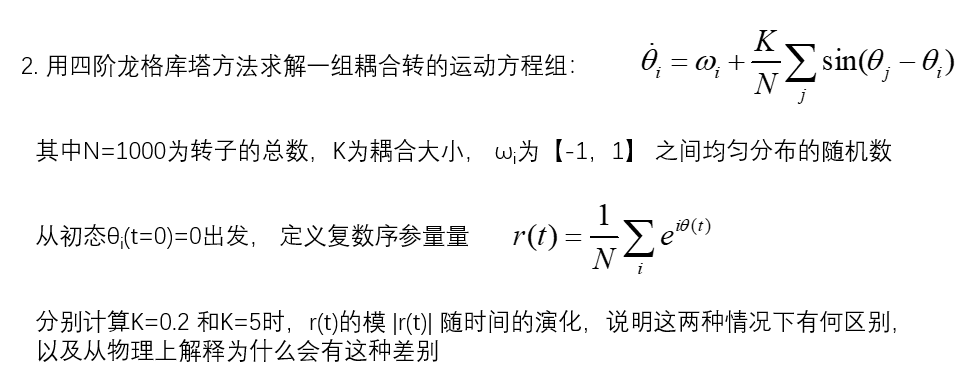
\includegraphics[width=1\textwidth,height=0.2\textwidth]{pictures/project2.png}
  \caption{题目总览} \label{project2}
\end{figure}
可以看出,这里需要解一个数量为1000的方程组。我们在解多阶微分方程的时候
对方程进行了化为方程组的思想方法,在这里我们就可以直接使用方程组的思想,
对于问题一中的情况稍作修改就可以得到同样有效的代码。\newline
\section{代码展示}
\subsubsection{前置函数编写}
以下为第二问所用到的微分方程,由于方程数量较多,所以我们采取循环的方式对方程组进行生成。\newline
~\\
\lstset{language=matlab}
\begin{lstlisting}
  function dtheta=fun(t,theta)
  w=2*rand([1,1000])-1;
  dtheta=zeros(1,1000);
  for ii=1:1000
      dtheta(ii)=w(ii)+0.2/1000*sum(theta-theta(ii));
  end
end
\end{lstlisting}
以下的编写思路和第一问是一样的,因为调用的变量为矩阵的行向量,因此可以便利地接受任意多的元素进行计算。\newline

~\\
\lstset{language=matlab}
\begin{lstlisting}
  function theta=rk(t,h,theta)
  len=length(t);
  for i=2:len
      K1=fun(t(i-1),theta(i-1,:));
      K2=fun(t(i-1)+1/2*h,theta(i-1,:)+1/2*h*K1);
      K3=fun(t(i-1)+1/2*h,theta(i-1,:)+1/2*h*K2);
      K4=fun(t(i-1)+h,theta(i-1,:)+h*K3);
      theta(i,:)=theta(i-1,:)+h/6.*(K1+2*K2+2*K3+K4);
  end
end
\end{lstlisting}
以下为绘图函数,使用求和函数后将其求模得到随时间变化的情况。\newline
~\\
\lstset{language=matlab}
\begin{lstlisting}
  function theta=PlotIt()
  t=0:0.01:50;
  h=t(2)-t(1);
  theta=zeros(length(t),1000);
  theta(1,:)=zeros(1,1000);%初始条件是所有转子起始位置为0
  Theta=rk(t,h,theta);
  hold on
  grid on
  r=zeros(1,length(t));
      for j=1:length(t)
          r(j)=1/1000*abs(sum(exp(1i*Theta(j,:))));
      end
  plot(t,r)
  end
\end{lstlisting}
\subsubsection{主体函数编写}
~\\
\lstset{language=matlab}
\begin{lstlisting}
  clear;clc;
  PlotIt()
\end{lstlisting}
本文中所例举的是K=0.2的情况,如果要得到K=5的情形只需要稍作修改即可。
\section{结果分析与结论}
\quad \newline
	\begin{figure}[!htbp]
		\centering
		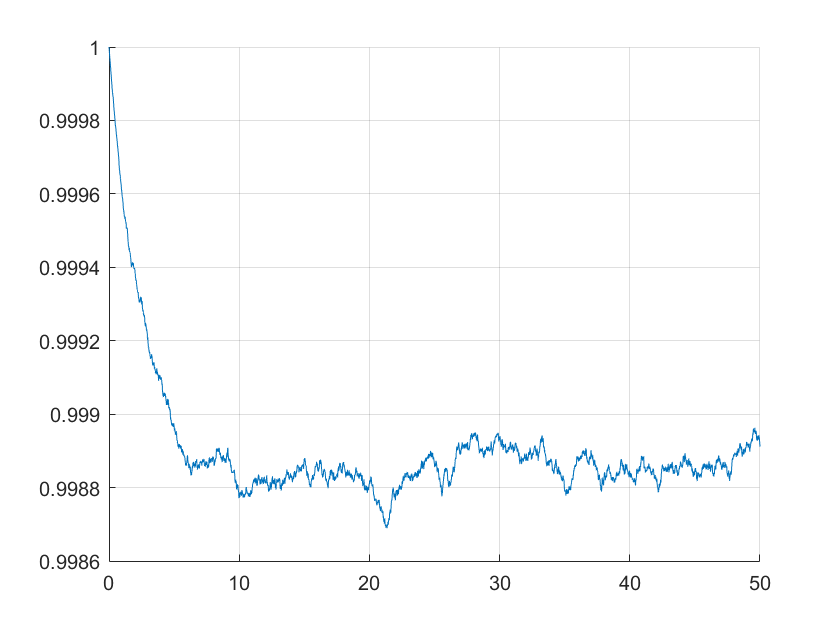
\includegraphics[width=0.6\textwidth,height=0.4\textwidth]{pictures/02.png}
		\caption{K=0.2} \label{02}
	\end{figure}
\quad \newline
	\begin{figure}[!htbp]
		\centering
		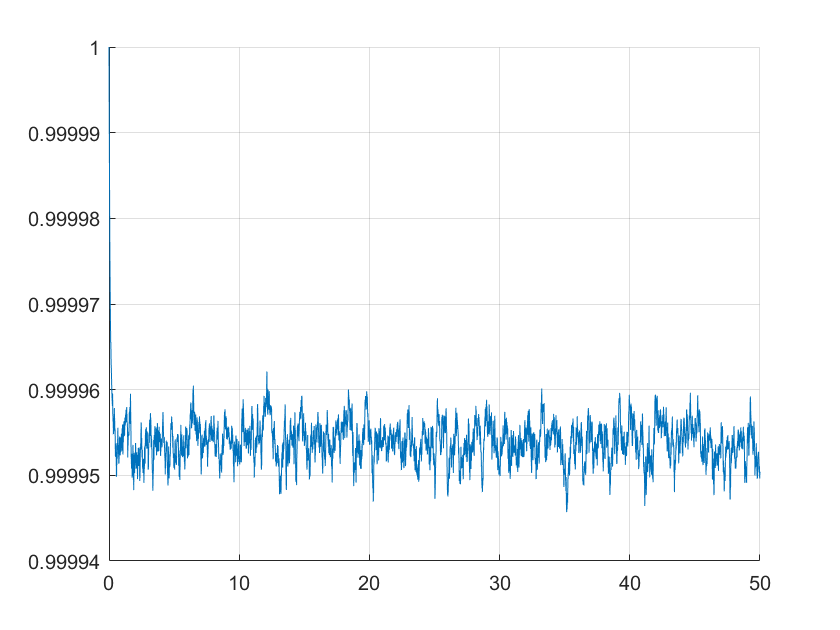
\includegraphics[width=0.6\textwidth,height=0.4\textwidth]{pictures/5.png}
		\caption{K=5} \label{5}
	\end{figure}

  通过观察我们可以发现,K=5的情况下,r函数以快得多的速度收敛到一个较为
  稳定的范围内。比如K=0.2时,大约到了t=10的时候r函数才开始出现振荡现象。
  而K=5的情况下就要快得多,大约在t=0.7的时候就进入了频率极高的振荡现象。\newline

  这是因为,K=5时转子们以更强的方式耦合在了一起,因此以很快的速度进行了同步。
%以下为插入代码模板
%~\\
%\lstset{language=matlab}
%\begin{lstlisting}
%\end{lstlisting}


%%%以下为插入图片模板
%\quad \newline
%	\begin{figure}[!htbp]
%		\centering
%		\includegraphics[width=0.5\textwidth,height=0.375\textwidth]{pictures/minscale.png}
%		\caption{最小风向} \label{minsacle}
%	\end{figure}

%%%以下为插入图片模板
%\quad \newline
%	\begin{figure}[!htbp]
%		\centering
%		\includegraphics[width=0.5\textwidth,height=0.375\textwidth]{pictures/minscale.png}
%		\caption{最小风向} \label{minsacle}
%	\end{figure}

%    \begin{algorithm}
%		\caption{Title of the Algorithm}
%     	\begin{algorithmic}[1]
%			\REQUIRE some words.  % this command shows "Input"
%			\ENSURE ~\\           % this command shows "Initialized"
%			some text goes here ... \\
%			\WHILE {\emph{not converged}}
%			\STATE ... \\  % line number at left side
%			\ENDWHILE
%			\RETURN this is the lat part.  % this command shows "Output"
%		\end{algorithmic}
%	\end{algorithm}

\end{document}